\documentclass[12pt,a4paper]{article}
\synctex=1
\usepackage[utf8]{inputenc}
\usepackage[margin=1cm]{geometry}
\usepackage{graphicx}
%\usepackage{verbatim}
\usepackage{listings}
\usepackage{textcomp}
\usepackage{courier}
\usepackage{libertine}
\usepackage{pgfornament}
\usepackage{eso-pic}
\usepackage[hangul]{kotex}
\linespread{1.3}

\title{
	\centering
	\pgfornament[width=12cm,color=teal]{84}\\
	\vspace{1cm}
	\fontsize{50}{50} \selectfont {컴퓨터 그래픽스 입문}\\
		\pgfornament[width=12cm,color=teal]{88}\\
	\vfill}
\author{
	\LARGE
	\begin{tabular}{rl}
		\hline
		학번 : & 2016110056\\ 
		학과 : & 불교학부 \\
		이름 : & 박승원\\
		날짜 : & \today\\
		\hline
	\end{tabular}\vspace{2cm}
	\\

\includegraphics[width=0.5\textwidth]{logo.jpg}
	}
\date{}


\begin{document}
\maketitle
\pagenumbering{gobble}
\noindent
\lstset{language=C++, columns=flexible, tabsize=4, frame=shadowbox, showstringspaces=false, breaklines=true, upquote=true, basicstyle=\normalsize}

\section{Draw a cube}
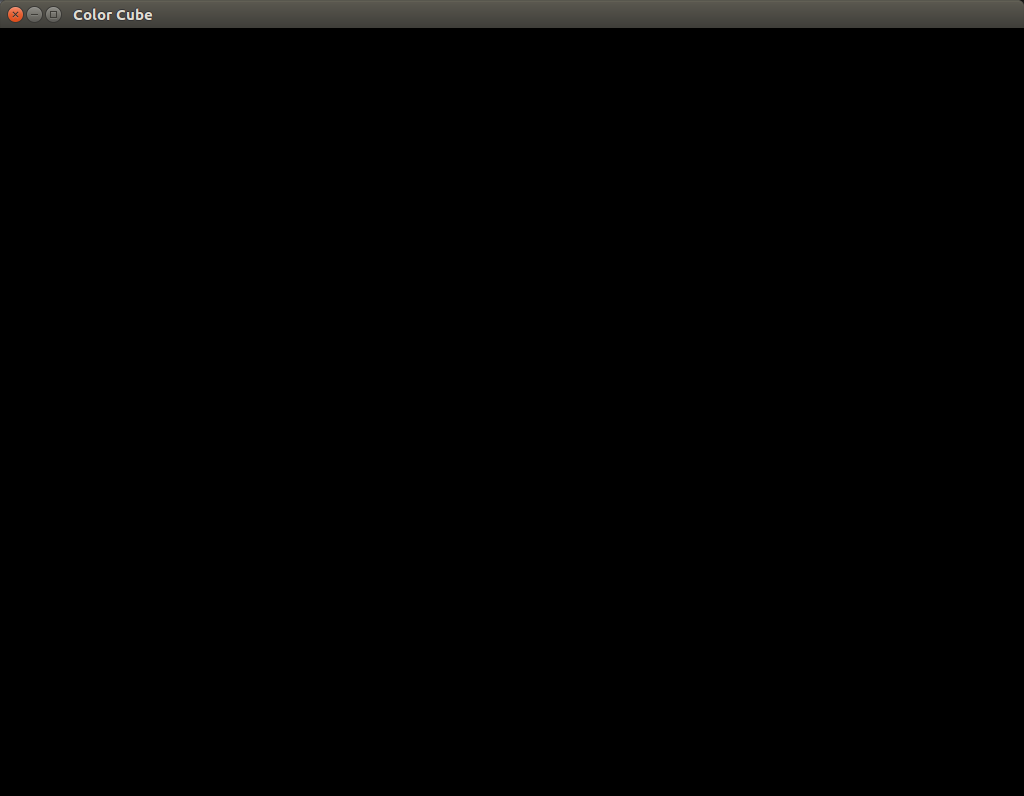
\includegraphics[width=\textwidth]{2.png}
\lstinputlisting{src/val.cpp}	
다각형을 만드는 polygon이란 함수를 이용했다.\\
이 함수는 다각형의 정점들을 반환한다.\\
육면체를 만들기 위해 4각형의 정점을 생성하고 이 점들을 Z축으로 이동시킨 4점을 추가하여 8개의 정점을 만든다.\\
8개의 정점들을 인덱스를 이용하여 4각형을 만들기 위한 순서로 다시 벡터에 입력한다.\\
색을 동일하게 하기 위해 valarray를 조작한다.\\
gltranferdata라는 함수는 벡터나 valarray를 이용하여 데이터를 보내고 리턴값으로 vbo를 받아온다.
\section{Draw a cone}
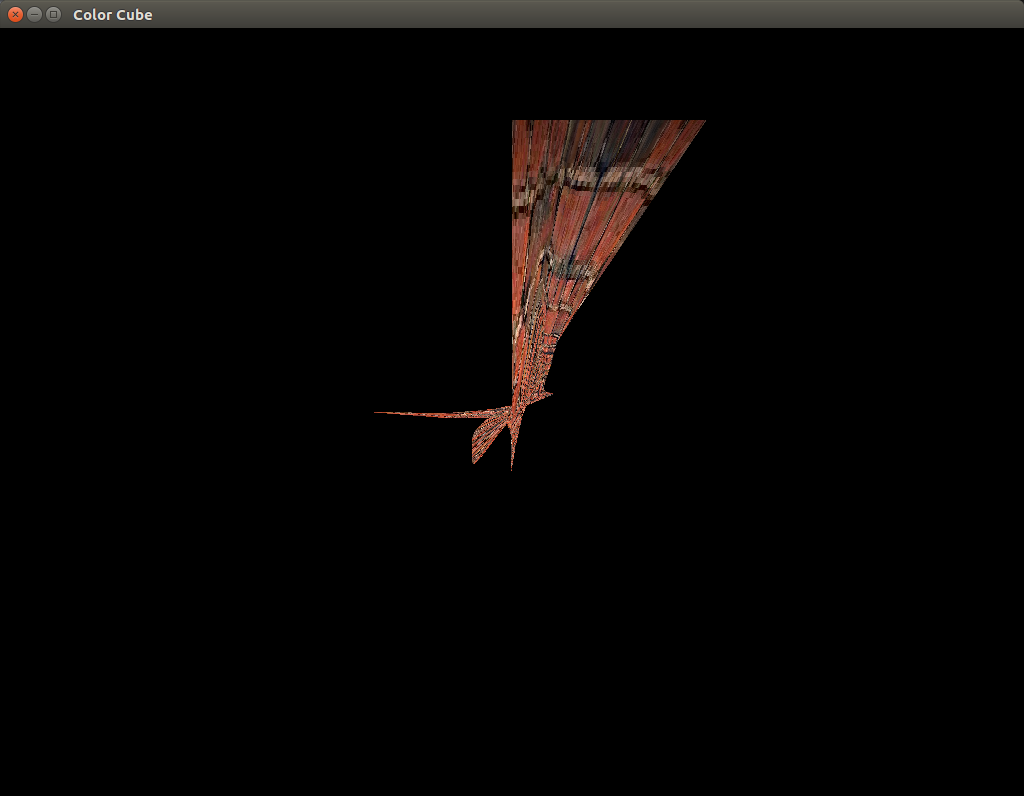
\includegraphics[width=\textwidth]{1.png}
\lstinputlisting{src/cone.cpp}	
polygon함수로 100각형을 생성한다. 인간의 눈에는 원으로 보인다.\\
앞 뒤에 원뿔의 꼭지점과 원의 시작점을 추가한다.\\
색의 데이터를 점의 데이터와 같게 하여 변화를 준다.\\

\lstinputlisting[caption=glutil.h]{src/glutil.h}

\lstinputlisting[caption=callbacks.cc : glutil implementation]{src/callbacks.cc}
	
\end{document}
